%% LyX 2.0.6 created this file.  For more info, see http://www.lyx.org/.
%% Do not edit unless you really know what you are doing.
\documentclass[12pt,english]{article}
\usepackage[T1]{fontenc}
\usepackage[latin9]{inputenc}
\usepackage{graphicx}

\makeatletter
%%%%%%%%%%%%%%%%%%%%%%%%%%%%%% User specified LaTeX commands.
\usepackage{graphicx}
\usepackage{amsmath}
\usepackage{amsfonts}
\usepackage{amssymb}
%TCIDATA{OutputFilter=latex2.dll}
%TCIDATA{CSTFile=LaTeX article (bright).cst}
%TCIDATA{Created=Thu Nov 06 21:35:40 2003}
%TCIDATA{LastRevised=Tue Nov 11 20:11:57 2003}
%TCIDATA{<META NAME="GraphicsSave" CONTENT="32">}
%TCIDATA{<META NAME="DocumentShell" CONTENT="General\Blank Document">}
%TCIDATA{Language=American English}
\newtheorem{theorem}{Theorem}
\newtheorem{acknowledgement}[theorem]{Acknowledgement}
\newtheorem{algorithm}[theorem]{Algorithm}
\newtheorem{axiom}[theorem]{Axiom}
\newtheorem{case}[theorem]{Case}
\newtheorem{claim}[theorem]{Claim}
\newtheorem{conclusion}[theorem]{Conclusion}
\newtheorem{condition}[theorem]{Condition}
\newtheorem{conjecture}[theorem]{Conjecture}
\newtheorem{corollary}[theorem]{Corollary}
\newtheorem{criterion}[theorem]{Criterion}
\newtheorem{definition}[theorem]{Definition}
\newtheorem{example}[theorem]{Example}
\newtheorem{exercise}[theorem]{Exercise}
\newtheorem{lemma}[theorem]{Lemma}
\newtheorem{notation}[theorem]{Notation}
\newtheorem{problem}[theorem]{Problem}
\newtheorem{proposition}[theorem]{Proposition}
\newtheorem{remark}[theorem]{Remark}
\newtheorem{solution}[theorem]{Solution}
\newtheorem{summary}[theorem]{Summary}
\newenvironment{proof}[1][Proof]{\textbf{#1.} }{\ \rule{0.5em}{0.5em}}

\makeatother

\usepackage{babel}
\begin{document}

\title{First Welfare Theorem in Production Economies}


\author{Michael Peters}


\date{\today{}}

\maketitle

\section{Profit Maximization}

Firms transform goods from one thing into another. If there are two
goods, $x$ and $y$, then a firm can transform $x$ into $y$ or
$y$ into $x$ depending on what consumers want. The first figure
below represents a simple production technology that the firms might
use to do this.
\begin{figure}
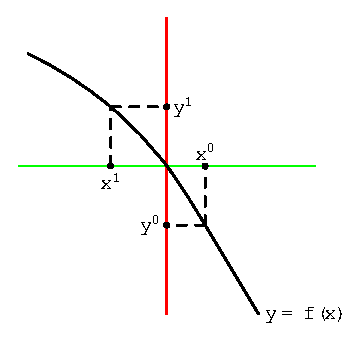
\includegraphics{firms_fig1}

\caption{Production Function\label{fig1}}
\end{figure}


In the figure, the function $y=f\left(x\right)$ represents the feasible
production choices available to the firm. The horizontal axis measures
an arbitrary good $x$ which could be either an input or an output.
When $x$ is negative, interpret this to mean that it is being used
as an input in the production of some good $y$ which is measured
along the vertical axis. Any good could be an input. For example some
firms use labor to produce parts for cars. The parts are an output
for that firm. The same parts act as an input for the firm that makes
cars. The distinction between inputs and outputs really isn't helpful
here. A better idea is to think of a production technology that can
transform one good into another. At a point on the production function
like $\left(x^{1},y^{1}\right)$, the firm transforms $x^{1}$ units
of good $x$ into $y^{1}$ units of good $y$. At this point, the
input $x$ is negative and the output $y$ is positive. On the other
hand, the firm could as easily use $y$ as an input ($y$ is negative)
and produce $x$ as an output as it does at the point $\left(x^{0},y^{0}\right)$. 

The way that firms are incorporated into things is to assume that
firms own all of the endowments of good $x$ and $y$. They transform
$x$ to $y$ or $y$ to $x$  in whatever way maximizes their profits.
Consumers, in turn, own firms. To make things simple, assume there
is only a single firm. There will also be two consumers, $1$ and
$2$. Let $\theta$ be the proportion of the firm owned by consumer
$1$ while $\left(1-\theta\right)$ is the proportion owned by consumer
$2.$ Let $\omega_{x}$ and $\omega_{y}$ be the total amounts of
good $x$ and $y$ that are available to the firm. 

Let $z_{x}$ and $z_{y}$ be the aggregate amounts of $x$ and $y$
that the firm chooses to make available in the economy. If the firm
decides that it wants to produce good $y$ from good $x$, meaning
that $z_{y}>\omega_{y}$ and $z_{x}<\omega_{x}$, then it needs to
use up some of its endowment of good $x$ and use it in production
of good $y$. So, $z_{y}=\omega_{y}+f\left(z_{x}-\omega_{x}\right)$.
(Remember that to get $y$ out of the production process, we need
a negative argument for good $x$ the way $f$ is drawn in Figure
$1$.) On the other hand, if it wants to produce good $x$ (that is
$z_{x}>\omega_{x}$), then it has to use up some of its endowment
of good $y$ (so, $z_{y}<\omega_{y}$). 

Now, imagine drawing a picture as in Figure $2$ of the function 
\begin{equation}
z_{y}=\omega_{y}+f\left(z_{x}-\omega_{x}\right)\label{ppf}
\end{equation}
 This function is called the \textit{production possibilities frontier}.
It is given as the line segment $CD$ in Figure 2. The output of good
$y$ varies between $\omega_{y}+f(\omega_{x})$ when the amount of
good $x$ the firm chooses to produce is 0, to $0$ in the case where
the firm chooses to produce an output $z$ such that $f(z-\omega_{x})+\omega_{y}=0$. 

Now, suppose that the prices for $x$ and $y$ are given by $p$ and
$1$, respectively (I keep using $1$ for the price of $y$ because
it is only the relative price of good $x$ that makes a difference
to the firm or the consumers). Whatever the firm chooses to produce
it can sell to the consumers at prices $p$ and $1$. So, the profit,
or revenue, of the firm is just $pz_{x}+z_{y}$, if it produces $\left(z_{x},z_{y}\right)$.
An iso-profit locus is a collection of productions that give the same
profit. The line segment $AB$ in Figure $2$ gives part of one such
production locus. There are a family of such loci--all of the lines
that are parallel to $AB$. If the firm maximizes profits, it picks
the highest iso-profit curve that touches its production possibilities
frontier. This gives the production choice $\left(z_{1},z_{2}\right)$
in Figure $2$. 

Once the firm has produced this output, it distributes its profits
back to its shareholders: the fraction $\theta$ goes to consumer
$1$, and $\left(1-\theta\right)$ goes to consumer $2$. Since the
consumers use these profits to finance their purchases, both of them
would prefer that the firm choose the aggregate production that maximizes
its profits since that will always provide them with their highest
income for consumption. The income of consumer $1$ is $\theta\left(pz_{1}+z_{2}\right)$.
This means that the budget line that consumer $1$ faces is the one
that intersects the $x$-axis at the point $\theta\left(pz_{1}+z_{2}\right)/p$
(since that is the maximum quantity of good $x$ he would be able
to purchase with that income). 

The outcome at an \emph{arbitrary} (i.e. not equilibrium) price pair
$\left(p,1\right)$ is given in Figure $2.$
\begin{figure}
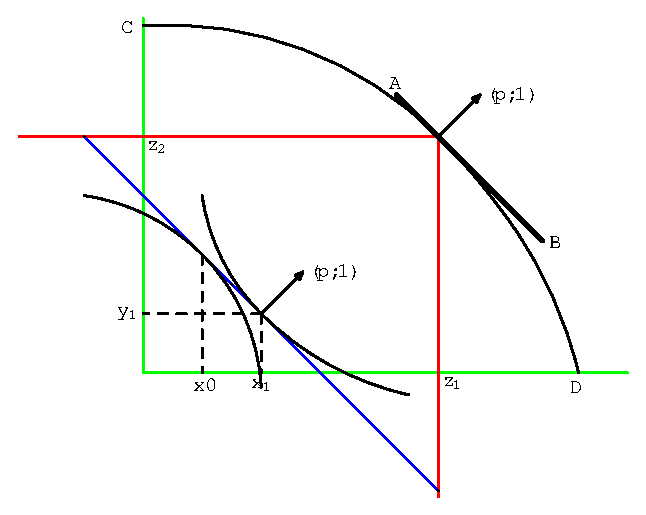
\includegraphics{firms_fig2}

\caption{Out of Equilibrium\label{fig2}}
\end{figure}


Each of the two consumers chooses the best point in his or her budget
set (which occurs where their indifference curves are tangent to their
corresponding budget lines). The choice by consumer $1$ is the consumption
bundle $\left(x_{1},y_{1}\right)$ in the figure. Consumer $2$'s
choice should be read with respect to the coordinate system that starts
at the point $\left(z_{1},z_{2}\right)$. So, the quantity of good
$x$ that consumer $2$ wants is given by the horizontal distance
between the point $x^{\prime}$ and the point $z_{1}$. From this,
you can see that the total demand for good $x$ (which is given by
$x_{1}+\left(z_{1}-x^{\prime}\right)$) exceeds the total amount of
good $x$ that is produced by the firm. So, the relative price of
$x$ should rise. 

As the relative price of $x$ rises, the family of iso-profit curves
faced by the firm will all get steeper. This will cause the firm to
choose a profit-maximizing level of output on its production possibilities
frontier that involves more $x$ and less $y$. As one might expect,
the rising price of good $x$ will cause both consumers to demand
a little less $x$ and a little more $y$. Eventually, the increase
in supply of $x$ and the reduction in demand will bring the market
to a state of equilibrium. 


\section{Competitive (Walrasian) Equilibrium}

A competitive (Walrasian) equilibrium is a pair of consumption choices
$\left(x_{1}^{\ast},y_{1}^{\ast}\right)$ for consumer $1$ and $\left(x_{2}^{\ast},y_{2}^{\ast}\right)$
for consumer $2$, and a production plan $\left(z_{1}^{\ast},z_{2}^{\ast}\right)$
for the firm such that there is a price $p^{\prime}$ for good $x$
for which the following things are true: 
\begin{enumerate}
\item $x_{1}^{\ast}+x_{2}^{\ast}=z_{1}^{\ast}$; $y_{1}^{\ast}+y_{2}^{\ast}=z_{2}^{\ast}$
(the markets clear); 
\item $p^{\prime}z_{1}^{\ast}+z_{2}^{\ast}\geq p^{\prime}z_{1}+z_{2}$ for
any pair $\left(z_{1},z_{2}\right)$ on the firm's production possibilities
frontier; and 
\item $u_{1}\left(x_{1}^{\ast},y_{1}^{\ast}\right)\geq u_{1}\left(x_{1},y_{1}\right)$
for all $\left(x_{1},y_{1}\right):p^{\prime}x_{1}+y_{1}\leq\theta\left(p^{\prime}z_{1}^{\ast}+z_{2}^{\ast}\right)$
and $u_{2}\left(x_{2}^{\ast},y_{2}^{\ast}\right)\geq u_{2}\left(x_{2},y_{2}\right)$
for all $\left(x_{2},y_{2}\right):p^{\prime}x_{2}+y_{2}\leq\left(1-\theta\right)\left(p^{\prime}z_{1}^{\ast}+z_{2}^{\ast}\right)$. 
\end{enumerate}
You can see what happens after the price of good $x$ rises (to $p^{\prime}$)
in Figure $3.$
\begin{figure}
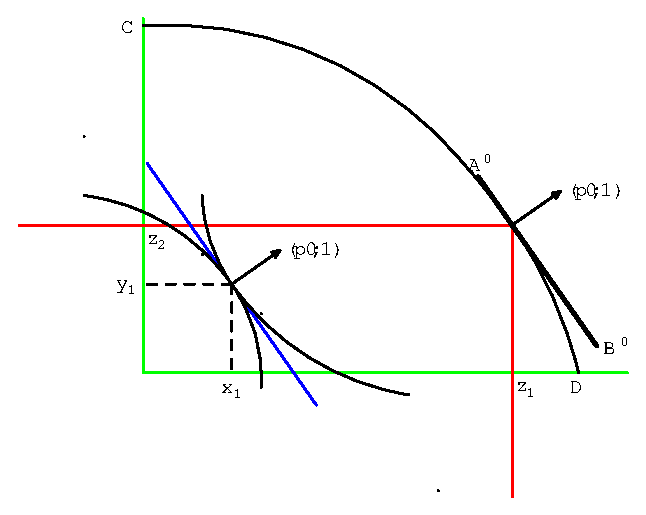
\includegraphics{firms_fig3}

\caption{Equilibrium\label{fig3}}
\end{figure}


In the picture, consumer $1$ now has income $\theta\left(p^{\prime}z_{1}^{\ast}+z_{2}^{\ast}\right)$
which he uses to buy $x_{1}^{\ast}$ units of good $x$. Now, consumer
$2$ chooses to buy $z_{1}^{\ast}-x_{1}^{\ast}$ units of good $x$,
and the markets clear. 


\section{First Welfare Theorem}

The \emph{first welfare theorem} is one of the most important contributions
of classical microeconomic theory. It says that no \emph{feasible}
allocation exists in which all consumers are better off than they
are in the competitive equilibrium. This is similar to the argument
that we made for an exchange economy: consumer indifference curves
must be tangent at any equilibrium. However, production adds another
wrinkle. It might be true that both consumers could be made better
off if the firm would just behave in a different fashion and pick
some production plan that doesn't necessarily maximize profits. 

Actually we can argue that if we take any pair of consumption bundles
where \emph{both} consumers are better off, then there can be no production
plan that makes this feasible. To see this, suppose that $\left(x_{1}^{\prime},y_{1}^{\prime}\right)$
and $\left(x_{2}^{\prime},y_{2}^{\prime}\right)$ are consumption
bundles such that
\[
u_{1}\left(x_{1}^{\prime},y_{1}^{\prime}\right)>u_{1}\left(x_{1}^{\ast},y_{1}^{\ast}\right)
\]
 and
\[
u_{2}\left(x_{2}^{\prime},y_{2}^{\prime}\right)>u_{2}\left(x_{1}^{\ast},y_{2}^{\ast}\right)
\]
 One observation is immediate. Whenever this is true, it must be that
\[
p^{\prime}x_{1}^{\prime}+y_{1}^{\prime}>\theta\left(p^{\prime}z_{1}^{\ast}+z_{2}^{\ast}\right)
\]
 and
\[
p^{\prime}x_{2}^{\prime}+y_{2}^{\prime}>\left(1-\theta\right)\left(p^{\prime}z_{1}^{\ast}+z_{2}^{\ast}\right)
\]
 The reason for this is that consumers choose the very best consumption
bundles that they can afford with their income. If they could have
afforded $\left(x_{1}^{\prime}.y_{1}^{\prime}\right)$ or $\left(x_{2}^{\prime},y_{2}^{\prime}\right)$,
then they certainly would have chosen them. 

Now, if the firm is maximizing its profits
\[
p^{\prime}z_{1}^{\ast}+z_{2}^{\ast}\geq p^{\prime}z_{1}^{\prime}+z_{2}^{\prime}
\]
 for any $\left(z_{1}^{\prime},z_{2}^{\prime}\right)$ along the firm's
production possibilities frontier. So, it must be that
\[
p^{\prime}x_{1}^{\prime}+y_{1}^{\prime}>\theta\left(p^{\prime}z_{1}^{\prime}+z_{2}^{\prime}\right)
\]
 and
\[
p^{\prime}x_{2}^{\prime}+y_{2}^{\prime}>\left(1-\theta\right)\left(p^{\prime}z_{1}^{\prime}+z_{2}^{\prime}\right)
\]
 Then, if we add these two inequalities together, we get
\[
p^{\prime}\left(x_{1}^{\prime}+x_{2}^{\prime}-z_{1}^{\prime}\right)+\left(y_{1}^{\prime}+y_{2}^{\prime}-z_{2}^{\prime}\right)>0
\]
 If prices are positive, then at least one of the two expressions
$\left(x_{1}^{\prime}+x_{2}^{\prime}-z_{1}^{\prime}\right)$ and $\left(y_{1}^{\prime}+y_{2}^{\prime}-z_{2}^{\prime}\right)$
are strictly positive, which means the firm simply can't produce enough
to supply what consumers want. 

So, it is good for firms to maximize profits in two senses. First,
if the firm were to propose some alternate production plan which didn't
involve profit maximization, both consumers would expect their income
to fall (notice that this is partly because they don't expect the
change in production plan to have any effect on prices). So, the shareholders
of the firm would unanimously vote against such a change. Second,
even if the firm could change its production plan, and even if prices
do change, the alternate plan can't possibly make both consumers better
off. Notice that when we make either of these arguments, we don't
value profits of firms for their own sake. We are only concerned with
the utility of consumers. 


\section{Distribution}

One thing you should notice about this entire construction is that
firms don't, in any sense, create wealth or goods. The ability to
create is embedded in the production possibilities frontier which
is taken as a given.%
\footnote{The traditional theory of the firm has nothing to say about where
this production possibilities frontier comes from. This makes it pretty
useless in thinking about things like economic development, or economic
growth.%
} All firms do is decide how to allocate this wealth. Many potential
ways to choose among alternate production plans exist. For example,
the government could choose the entire production plan. This was the
model used in centrally-planned economies like the old Soviet Union.
Alternatively, one could imagine a mixture of private, profit-maximizing
firms and publicly-regulated companies, similar to what happens in
most Western economies. 

Profit maximization isn't necessarily good for everyone. To see this,
consider the following example in which one of the consumers (say
consumer $1$) simply has an endowment of the goods $x$ and $y$
but does not own shares. The other, consumer 2, owns a firm that can
transform $x$ into $y$ (and conversely)-- possibly by buying some
of the endowment of consumer $1$. The firm that is owned by consumer
$2$ starts with some endowment of goods. 

To begin, suppose that the government declares that the firm is not
allowed to produce anything and that it simply has to give its endowment
to consumer $2$ who can use the endowment to finance the best consumption
plan possible. Restrictions like this are pretty common. An example
might be a zoning restriction that prevents a homeowner from turning
her house into an apartment building, or a farm owner who is not allowed
to build housing on his farm land. A possible outcome is shown in
Figure \ref{fig4}$.$
\begin{figure}
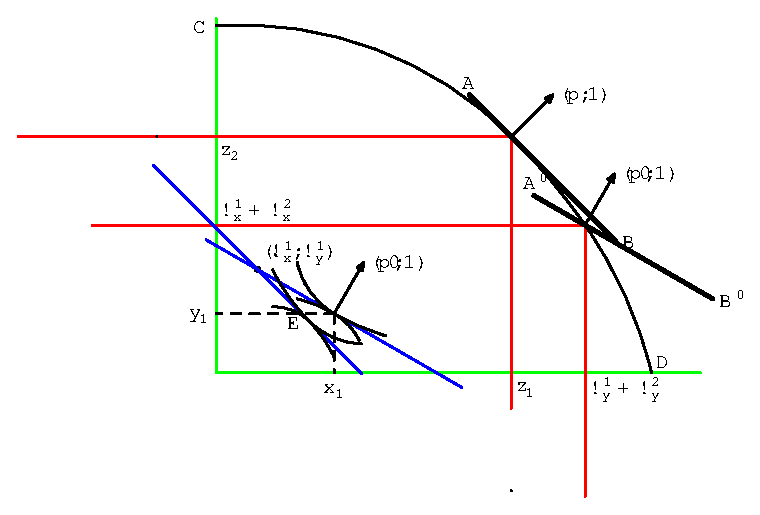
\includegraphics{firms_fig4}

\caption{Distribution\label{fig4}}
\end{figure}


In Figure $4$, consumer $1$ starts with an endowment equal to $\left(\omega_{x}^{1},\omega_{y}^{1}\right)$.
Consumer $1$ owns no shares of the firm. The firm owns an endowment
$\left(\omega_{x}^{2},\omega_{y}^{2}\right)$ and this firm is in
turn owned by consumer $2.$ If the firm simply offers its endowment
for sale on the market then the feasible set of trades is given by
the wide flat box whose corners are at the origin, and at the point
where the line segment $A^{\prime}B^{\prime}$ intersects the production
possibilities frontier. Prices adjust until the relative price of
$x$ is $p^{\prime}$. In the associated exchange equilibrium, consumer
$1$ receives the allocation $\left(x_{1}^{\ast},y_{1}^{\ast}\right)$.
Consumer $2$'s indifference curve is tangent to this point, so conditional
on the production decision of the firm, no allocation can make both
consumer $1$ and consumer $2$ better off. Notice that in this equilibrium,
consumer $1$ is selling some of his endowment of good $y$ in order
to acquire good $x$. Of course, consumer $2$ is doing the opposite:
selling off the good $x$ that the firm provides in order to acquire
good $y$. 

The iso-profit curves faced by the firm are all parallel straight
lines whose slopes are equal to $-p^{\prime}.$ Plotting the aggregate
endowment point on the production possibilities frontier shows that
simply selling off the endowment does not maximize the firm's profits.
The iso-profit line (with slope $-p$) is flatter than the production
possibilities frontier. Consumer $2$ will do better if the firm alters
its production plan to produce some additional $y$ from the endowment
of good $x$ because this will increase the income that consumer $2$
takes to the market. To put is in a slightly different way, observe
that the steep production possibilities curve means that consumer
$2$ can acquire good $y$ much more cheaply by having the firm produce
it than she can by buying it from consumer $1$. 

If the firm is now free to raise its output of $y$, it will create
an excess supply of good $y$ that will make $y$'s relative price
fall, or make $x$'s relative price rise. Both these things are bad
for consumer $1$ who is buying $x$ and selling $y$. When markets
finally clear, the relative price of good $x$ will level off at $p$,
and consumer $1$ will end up at point $E$ where he is much worse
off than he was in the original equilibrium. 

Oddly enough, this new equilibrium is \emph{Pareto optimal}. There
is no way to make \emph{both of the consumers} better off by changing
the firm's production plan. How does one reconcile this with the fact
that consumer $1$ was so much better off in the original equilibrium? 

One possible answer that may have occurred to you is that the original
equilibrium is also Pareto optimal. This is partly right and partly
wrong. The absolute value of the slope of the production possibilities
curve, at the point where the iso-profit curve $A^{\prime}B^{\prime}$
crosses it, is called the \emph{marginal rate of transformation} between
$x$ and $y$. If you think of using one small unit $dx$ of $x$
as the input, then the slope gives the amount of $y$ that you get
back out for each such unit. At the point $\left(x_{1}^{\ast},y_{1}^{\ast}\right)$
where the indifference curves for the consumers are tangent, the indifference
curves both have slope $-p^{\prime}$. The absolute value of this
is less than the marginal rate of transformation along the production
possibilities frontier. 

So, what is the slope of consumers $1$'s indifference curve? His
marginal rate of substitution is the amount of good $y$ you would
need to give him to compensate him when you take away a little ($dx$)
of his good $x$. Consumer $2$'s indifference curve is tangent at
this point. That means if you do a tiny transfer of good $x$, say
$dx$, from consumer $1$ to consumer $2$, and consumer $2$ compensates
$1$ by giving him $dy$ in exchange, where $dy$ is $1$'s (and $2$'s)
marginal rate of substitution, neither $1$ or $2$ are any better
off. 

Instead of transferring good $x$ from consumer $2$ to consumer $1$,
suppose that $1$ transfers a tiny bit of good $x$ to $2$ who uses
it to produce additional $y$ using the production function. The production
possibilities frontier is steeper than $1$'s indifference curve,
so this will give $2$ more than enough output to pay $1$ his marginal
rate of substitution and maintain his utility. But then, all the residual
output will be left over for consumer $2$ to enjoy. In other words,
when the production possibilities frontier is steeper than both consumer's
indifference curves, 2 can take a little of $1$'s good $x$ and use
it to produce $y$, which he uses to pay $1$ back for the good $x$.
Then, $2$ will have some output left over for himself. The endowment
point can't be Pareto optimal. 

On the other hand, if Pareto optimality is the only objective, it
can be achieved at the initial endowment point simply by moving along
the contract curve until the consumers' marginal rates of substitution
are equal to the marginal rate of transformation in production. Figure
5 shows how this might be accomplished.
\begin{figure}
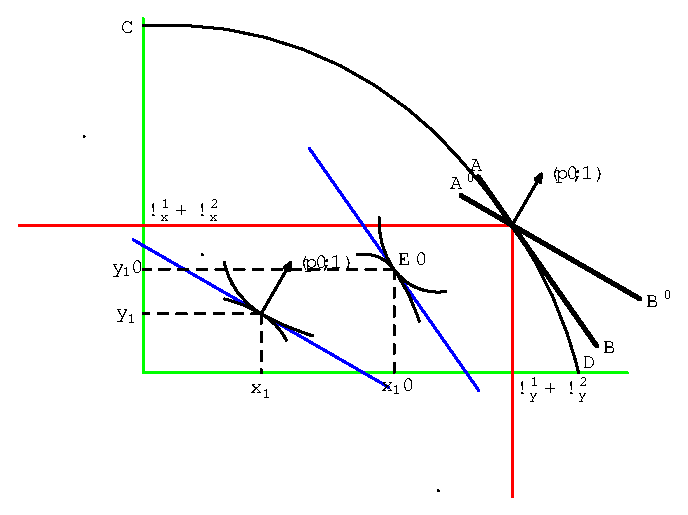
\includegraphics{firms_fig5}

\caption{An Alternative \label{fig5}}
\end{figure}


Notice that at the point $E^{\prime}$ in Figure $5$, the indifference
curves are both tangent and have the same slope as the production
possibilities curve at the endowment point. So, everything is Pareto
optimal. This might be achieved by having the government regulate
the firm's output choice, tax away some of the firm's profit (a tax
on dividends or capital gains) and then redistribute the proceeds
to consumer $1$. Consumer $1$ will love this alternative plan, and
consumer $2$ will hate it, but it will produce a Pareto optimal outcome. 

Pareto optimality is a perfectly sensible objective for economic policy
to try to accomplish. Profit maximization by firms is one way to achieve
this, but you need to remember that it is a means to a goal, not a
goal in itself. You should also try to remember, as Figure $5$ illustrates,
that there are alternative ways of achieving Pareto optimality. Different
methods lead to different distributional consequences - so, even though
all consumers will agree that they want the outcome to be Pareto optimal,
they may sensibly disagree about how this is accomplished. 
\end{document}
